\chapter{Fejlesztői dokumentáció} 
\label{ch:impl}

Az alkalmazás \textbf{Microsoft Visual Studio} segítségével készült. A kódok elsősorban C++, másodsorban -- a shaderek -- GLSL nyelven íródtak. Ha újra akarnánk fordítani akkor a \textbf{C:/} helyre csomagoljuk ki a mellékelt OGLPack.zip állományt (ez az szükséges csomagokat és függőségeket tartalmazza), majd futtassuk a \textbf{subst T: C:/} parancsot. Ezután megnyithatjuk a \textbf{.vcxproj} projektfájlt.

\section{Fejlesztői eszközök}

A program írása során számos könyvtár és API felhasználásra került. Ebben az alfejezetben ezek kerülnek bemutatásra.

\subsection{Simple DirectMedia Layer (SDL)}
A Simple DirectMedia Layer (SDL) könyvtár egy crossplatform multimédiás könyvtár, ami alacsony szintű, hatékony hozzáférést ad audio, bemeneti (egér, billentyűzet, joystick), valamint grafikus (OpenGL-en keresztül GPU-hoz) eszközökhöz. Az alkalmazásban az SDL 2.0 van használva. \cite{SimpleDi88:online}

\begin{figure}[H]
	\centering
	
\includegraphics[width=0.5\textwidth]{Sdl}
	\caption{Az SDL logója}
	\label{fig:Opengl}
\end{figure}

\subsection{OpenGL API}
Az OpenGL (Open Graphics Library) egy részletesen kidolgozott szabvány, melyet a Silicon Graphics nevű amerikai cég fejlesztett ki 1992-ben. Olyan API-t takar, amely segítségével egy egyszerű, szabványos felületen keresztül megvalósítható a grafikus kártya kezelése és a háromdimenziós grafika programozása. Az interfész több ezer különböző függvényhívásból áll, melynek segítségével a programozók szinte közvetlenül vezérelhetik a grafikus kártyát, segítségükkel 3 dimenziós alakzatokat rajzolhatnak ki, és a kirajzolás módját szabályozhatják. \cite{OpenGL–W93:online} 

\begin{figure}[H]
	\centering
	
\includegraphics[width=0.5\textwidth]{Opengl}
	\caption{Az OpenGL logója}
	\label{fig:Opengl}
\end{figure}

\subsection{Dear ImGui}
A \textbf{``Parameters''} feliartú panel megjelenítése ennek segítségével lett megoldva. A Dear ImGui (ImGui) egy egyszerű grafikai interfész könyvtár C++ nyelvhez. Segítségével egyszerűen kezelhetünk gombokat, csúszkákat, egyéb beviteli eszközöket valamint könnyen megjeleníthetünk adatokat. Gyors és hordozható, nincs szükség külső könyvtára csak néhány szimpla forrás fájl beillesztésére. \cite{ocornuti13:online}

\subsection{GLM}

Az OpenGL Mathematics egy headerben importálható C++ könyvtár mely a GLSL specifikációira szabva (elnevezések, funkciók) tartalmaz számtalan matematikai funkciót. Segítségével a GLSL-ben használatos funkciók és típusok C++-ban is használhatóak. \cite{OpenGLMa34:online}

\begin{figure}[H]
	\centering
	\includegraphics[width=0.5\textwidth]{GLM}
	\caption{A GLM logója}
	\label{fig:GLM}
\end{figure}

\section{Képalkotási módszer}
A megjelenítés \textbf{Raycast} technika (\ref{fig:trace_diag}.~ábra) alkalmazásával történik, egy speciális implicit reprezentáción, a távolságfüggvényeken. Ehhez minden pixelre ki kell számolni egy sugár paramétereit. Ezen sugár és felület metszetét a \textbf{Sphere tracing} algoritmussal kapjuk meg. A felületi normálist numerikusan számítjuk ki, melynek segítségével a felület már könnyen árnyalható.

\begin{figure}[H]
	\centering
	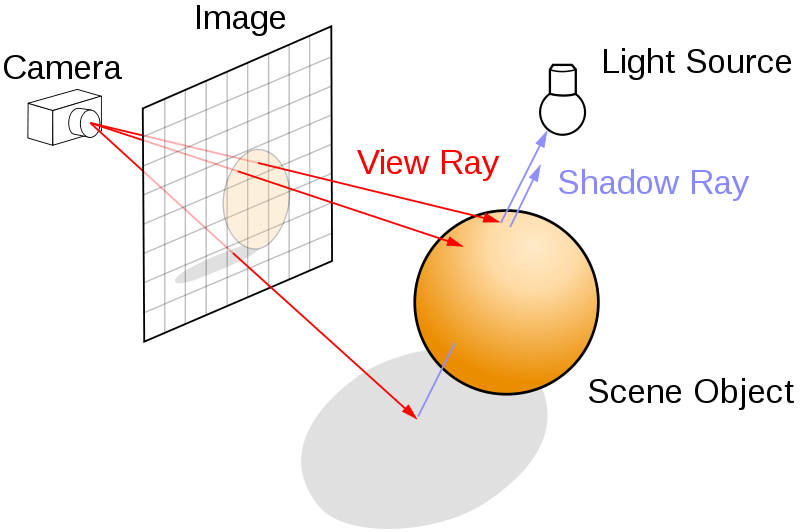
\includegraphics[width=0.5\textwidth]{trace_diag}
	\caption{A raycast technika ábrázolása. \cite{FileRayt97:online}}
	\label{fig:trace_diag}
\end{figure}

A \textbf{sphere tracing} algoritmus egy speciális esete az úgynevezett \textbf{raymarching} algoritmusnak. Működéséhez a kirajzolni kívánt objektumokat távolságfüggvényekkel kell reprezentálni, mely a virtuális tér bármely pontjáról képes meghatározni hogy milyen messze van az objektum felületétől. Az algoritmus egy implementációja \aref{src:raymarch}. forráskód részletben látható.

\lstset{caption={A sphere tarcing algoritmust megvalósító kód}, label=src:raymarch}
\begin{lstlisting}[language={C++}]
float RayMarch(vec3 ro, vec3 rd) {
	float dist=0.0;    
    for(int i=0; i<MAX_STEPS; i++) {
    	vec3 p = ro + rd*dist;
        float dS = GetDist(p);
        dist += dS;
        if(dist>MAX_DIST || dS<SURF_DIST ) break;
    }    
    return dist;
}
\end{lstlisting}

Az algoritmus két paramétert igényel: egy pontot és egy vektort, melyek meghatározzák a sugár kezdőpontját ér irányát. Ezen irány mentén lépked folyamatosan mindig annyit amennyit amekkora a távolság a legközelebbi felülethez képest. Ezt addig csinálja míg már kellően közel lesz (dS<SURF\_DIST), vagy ha már túl messzire ment (dist>MAX\_DIST), vagy esetleg túl sokat lépett (i>MAX\_STEP). 


\begin{figure}[H]
	\centering
	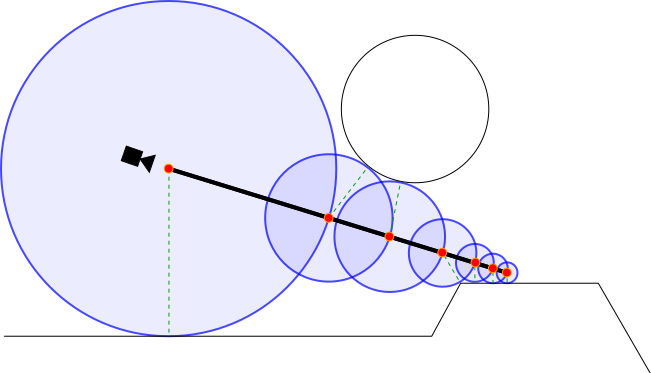
\includegraphics[width=0.4\textwidth]{SphereTracing}
	\caption{Sphere tracing: A kamerából kiinduló fénysugár mindig csak annyit halad előre amekkora a hozzá legközelebb lévő felület távolsága \cite{Raymarch94:online}}
	\label{fig:SphereTracing}
\end{figure}

Az alkalmazásban teljesítményjavítás érdekében másik feltétel (dS<0.01*dist/MAX\_DIST) lett használva a felületi távolsághoz, mely számításba veszi hogy mennyire messzire vagyunk a kamerától. Ha messzebb vagyunk akkor nincsen szükség akkora részletességre és a felületi távolság így lehet nagyobb is.

\subsection{Fénymodell}

Ha túl messzire ment a sugarunk (dist>MAX\_DIST), akkor egyszerűen a háttér színét adjuk a pixelnek. Egyéb esetben pedig kiszámoljuk az adott pontban a felületi normálist és a fénymodell segítségével megállapítjuk a pixel színét.

A használt fénymodell nagyon sokat számít a kirajzolt kép minőségén. Ezért sok idő és energia lett rászánva ennek megalkotására. Ezen fénymodell komponensei \aref{fig:lighting}.~ábrán láthatóak. Ezek különböző színenkénti súlyozással vett összege alkotja végső színáranyalatot, melyre még egy gamma korrekció és egy ködszerű effekt is került -- ez utóbbi arra szolgál hogy a viszonylag kicsi maximális távolságot leplezze.

\begin{figure}[H]
	\centering
	\subfigure[Objektumok alapszíne]{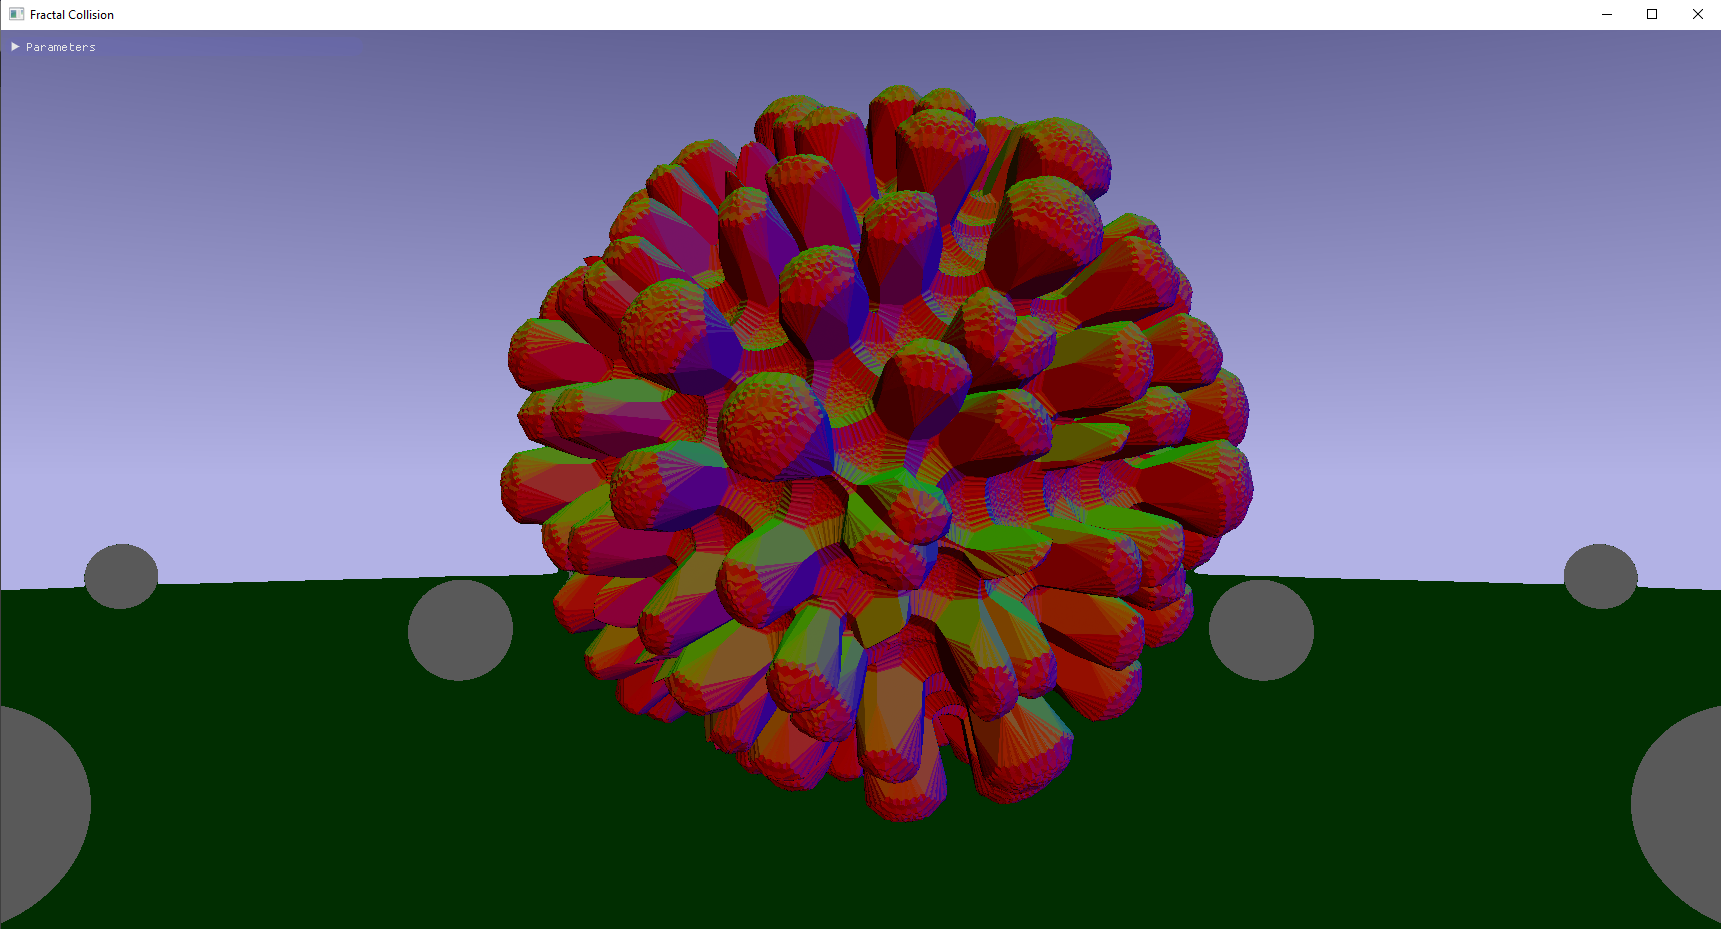
\includegraphics[width=0.3\linewidth]{col}}
	\hspace{1pt}
	\subfigure[Módosított ambiens fény]{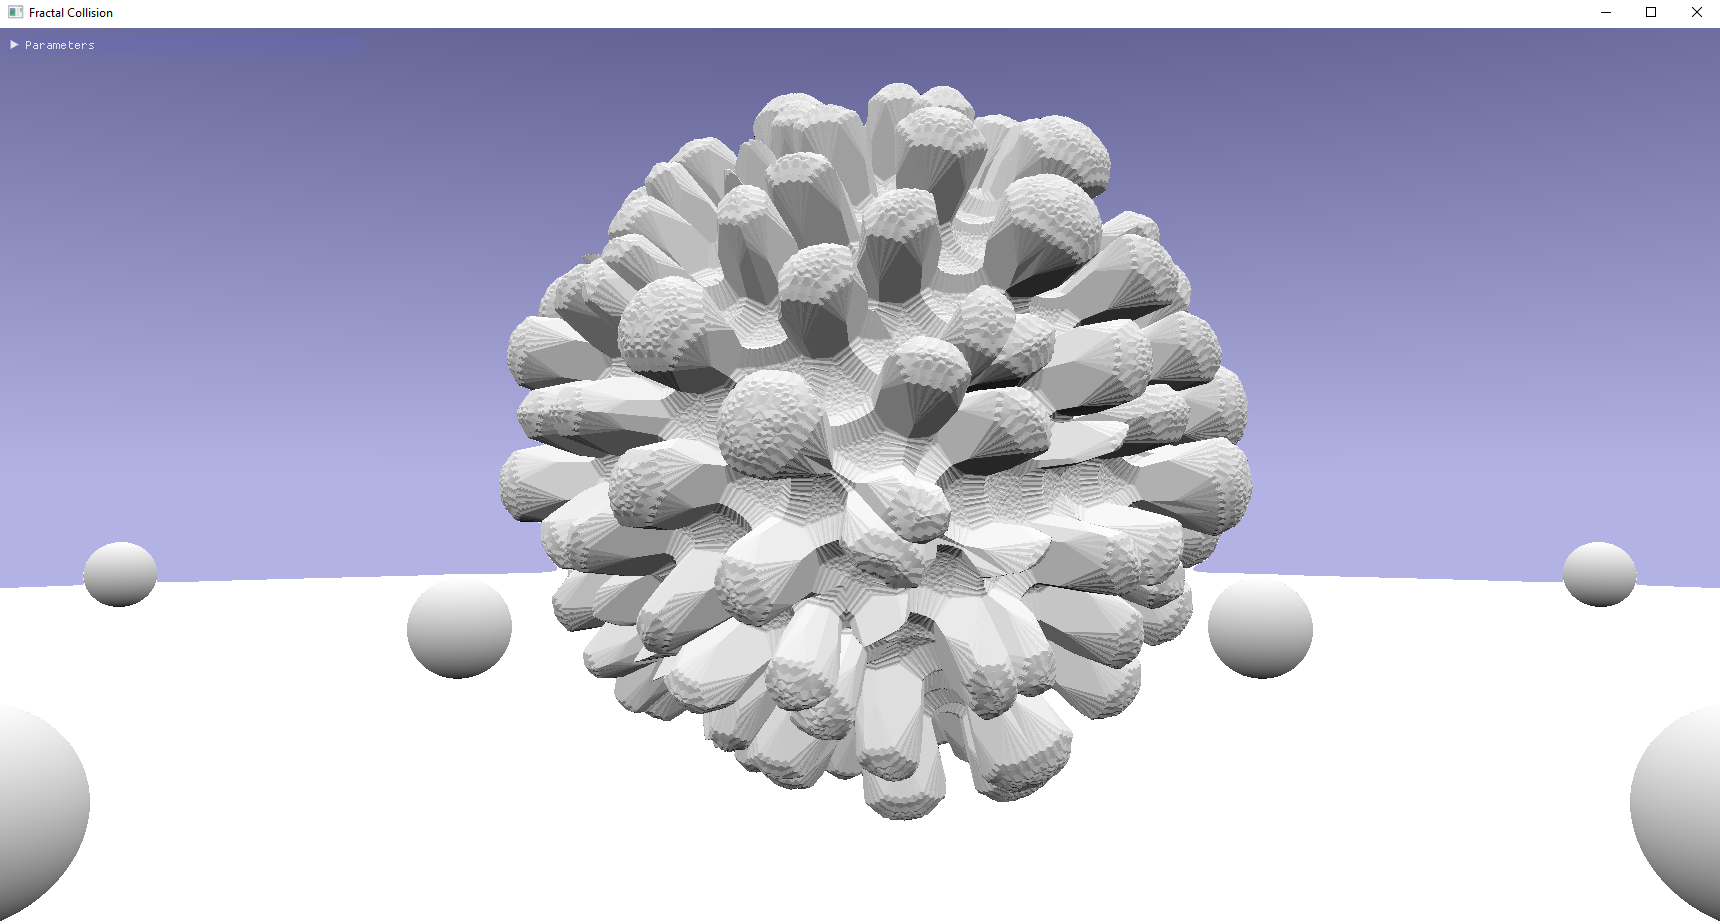
\includegraphics[width=0.3\linewidth]{amb}}
	\hspace{1pt}
	\subfigure[Ambiens eltakarás]{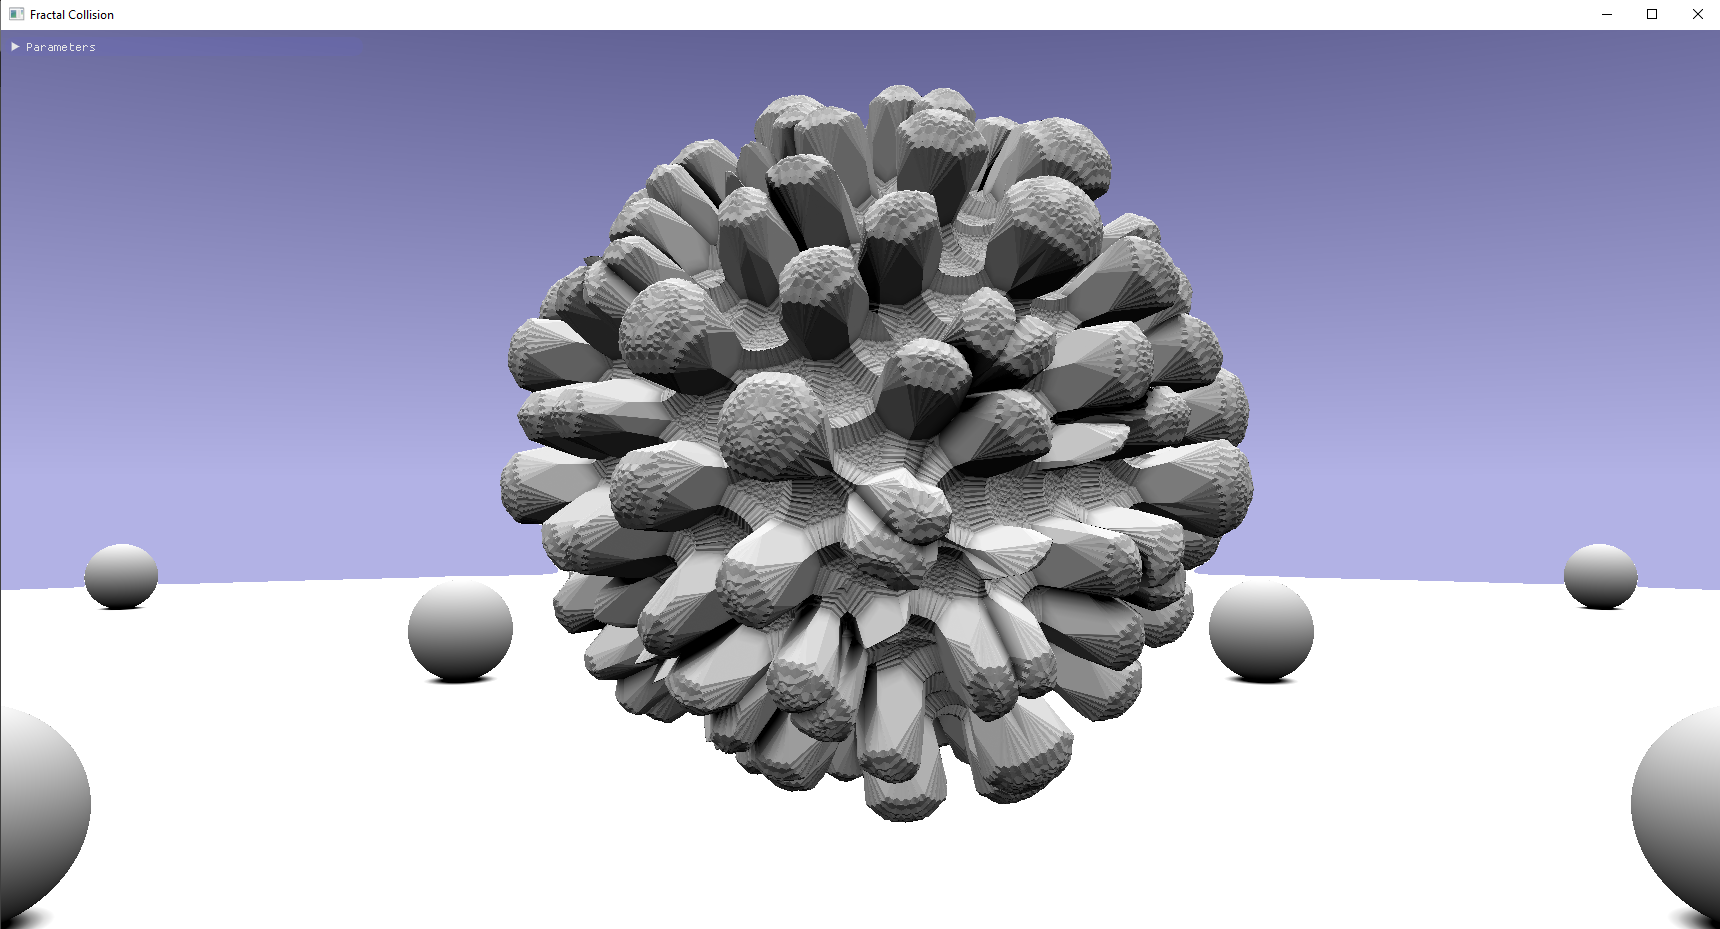
\includegraphics[width=0.3\linewidth]{occ}}
	\vspace{1pt}
	\subfigure[Spekuláris]{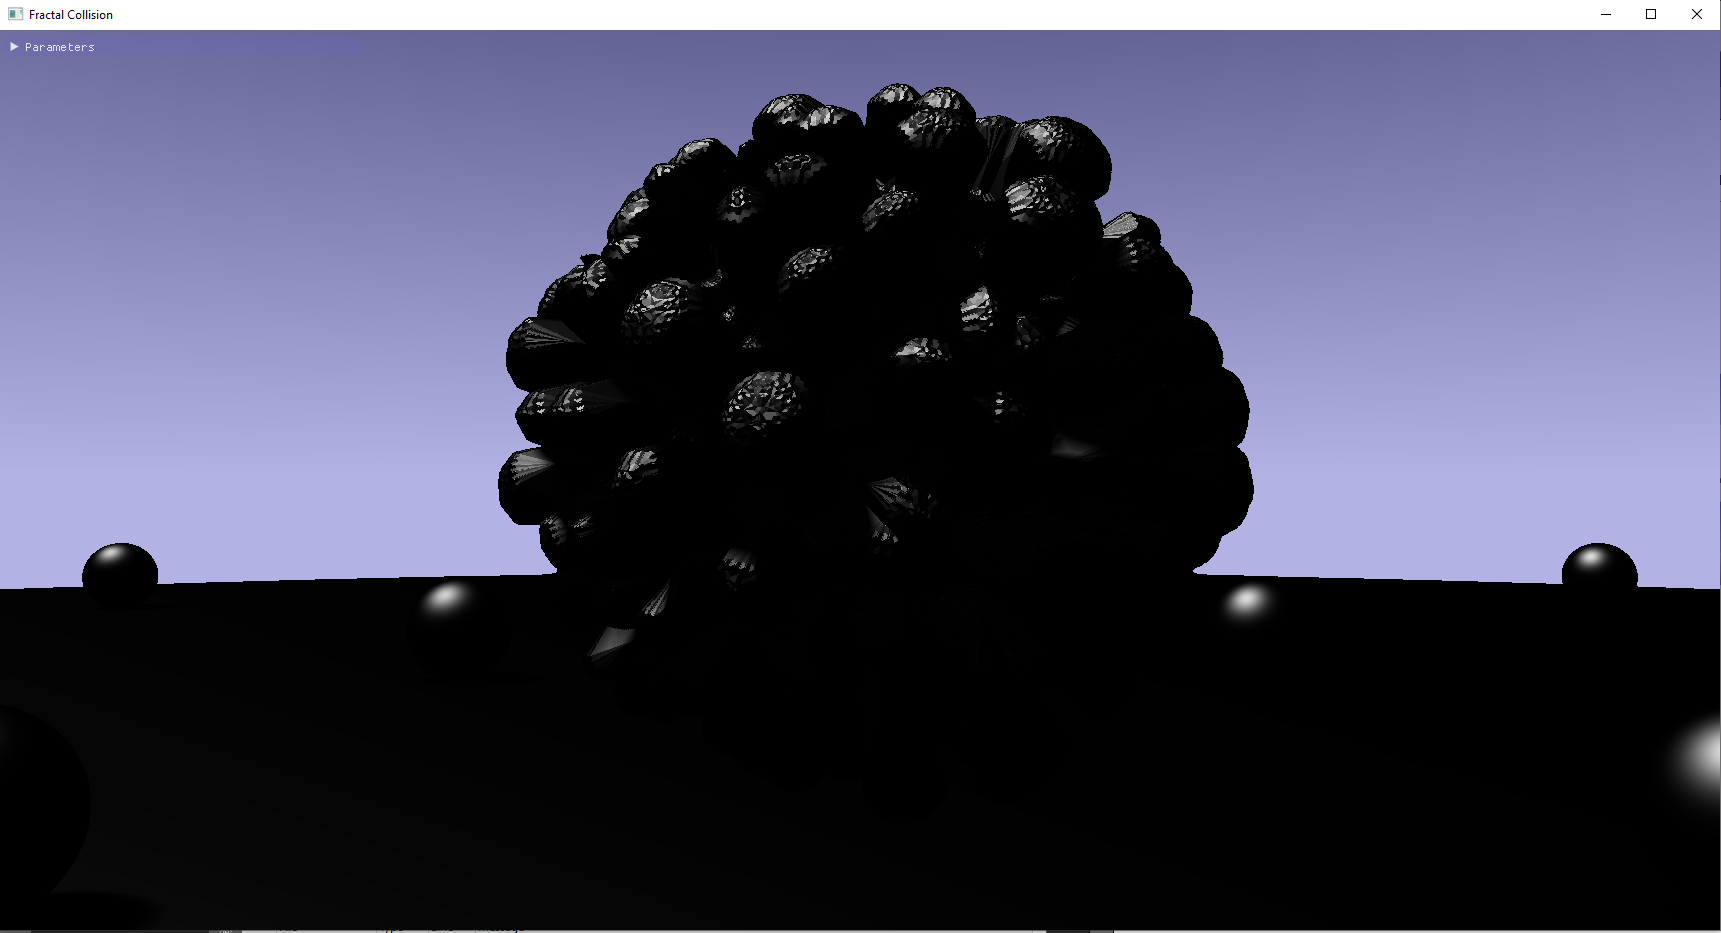
\includegraphics[width=0.3\linewidth]{spe}}
	\hspace{1pt}
	\subfigure[Diffúz * Árnyék]{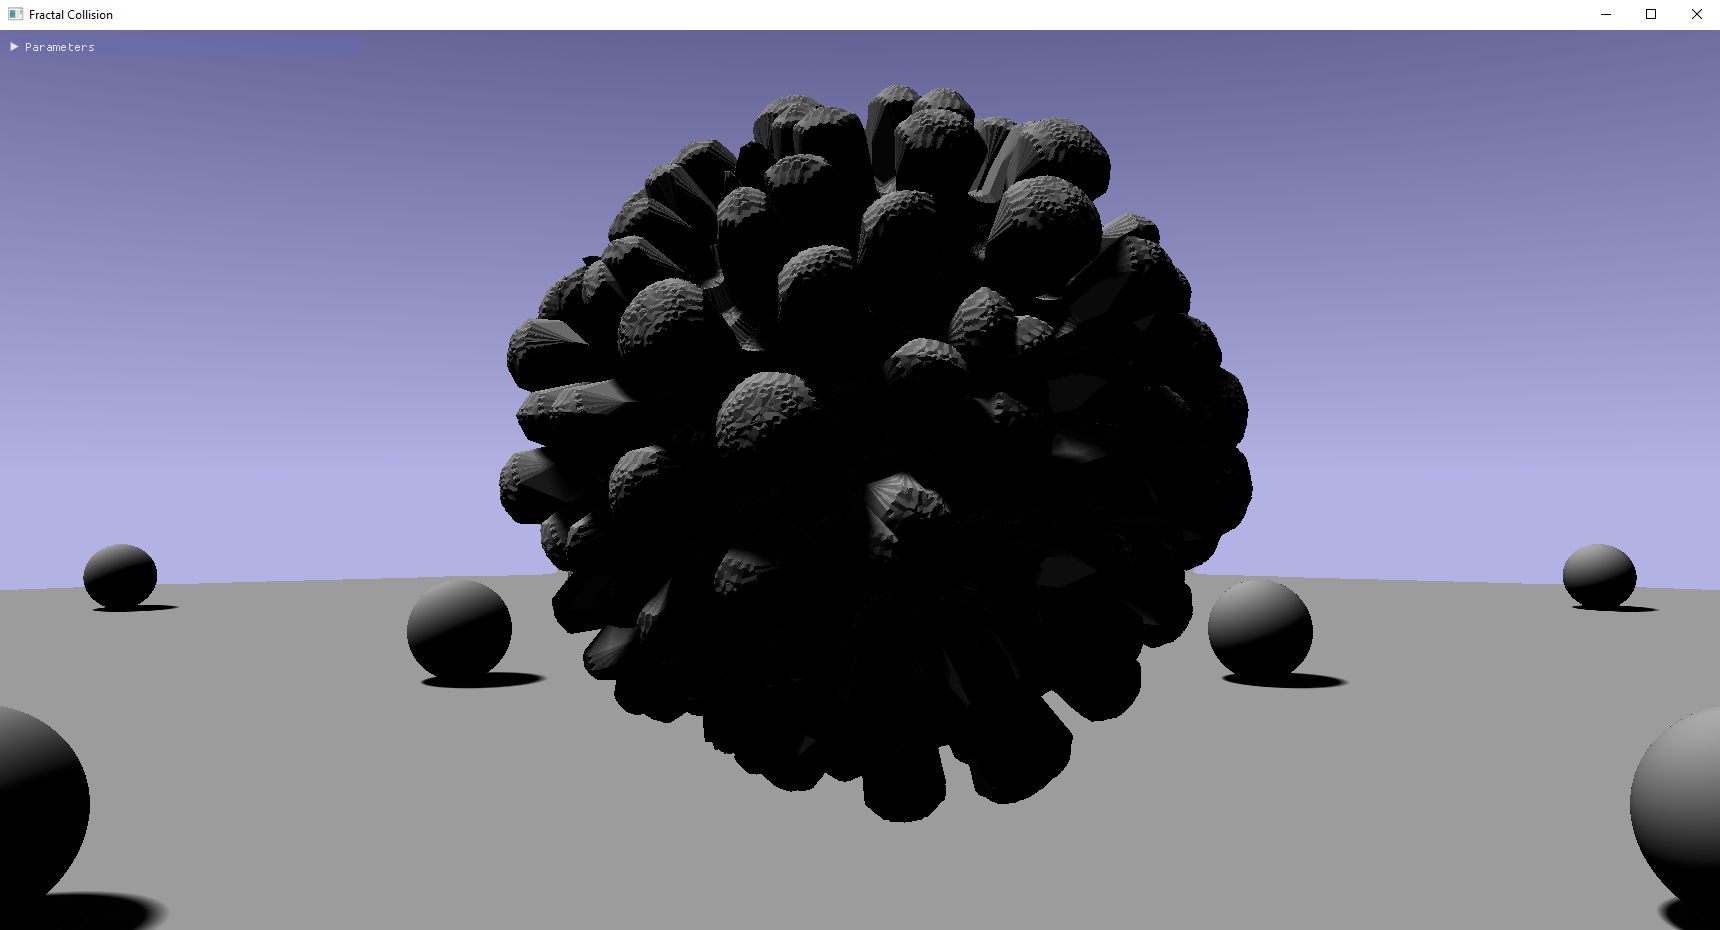
\includegraphics[width=0.3\linewidth]{shadif}}
	\hspace{1pt}
	\subfigure[Ellenfény]{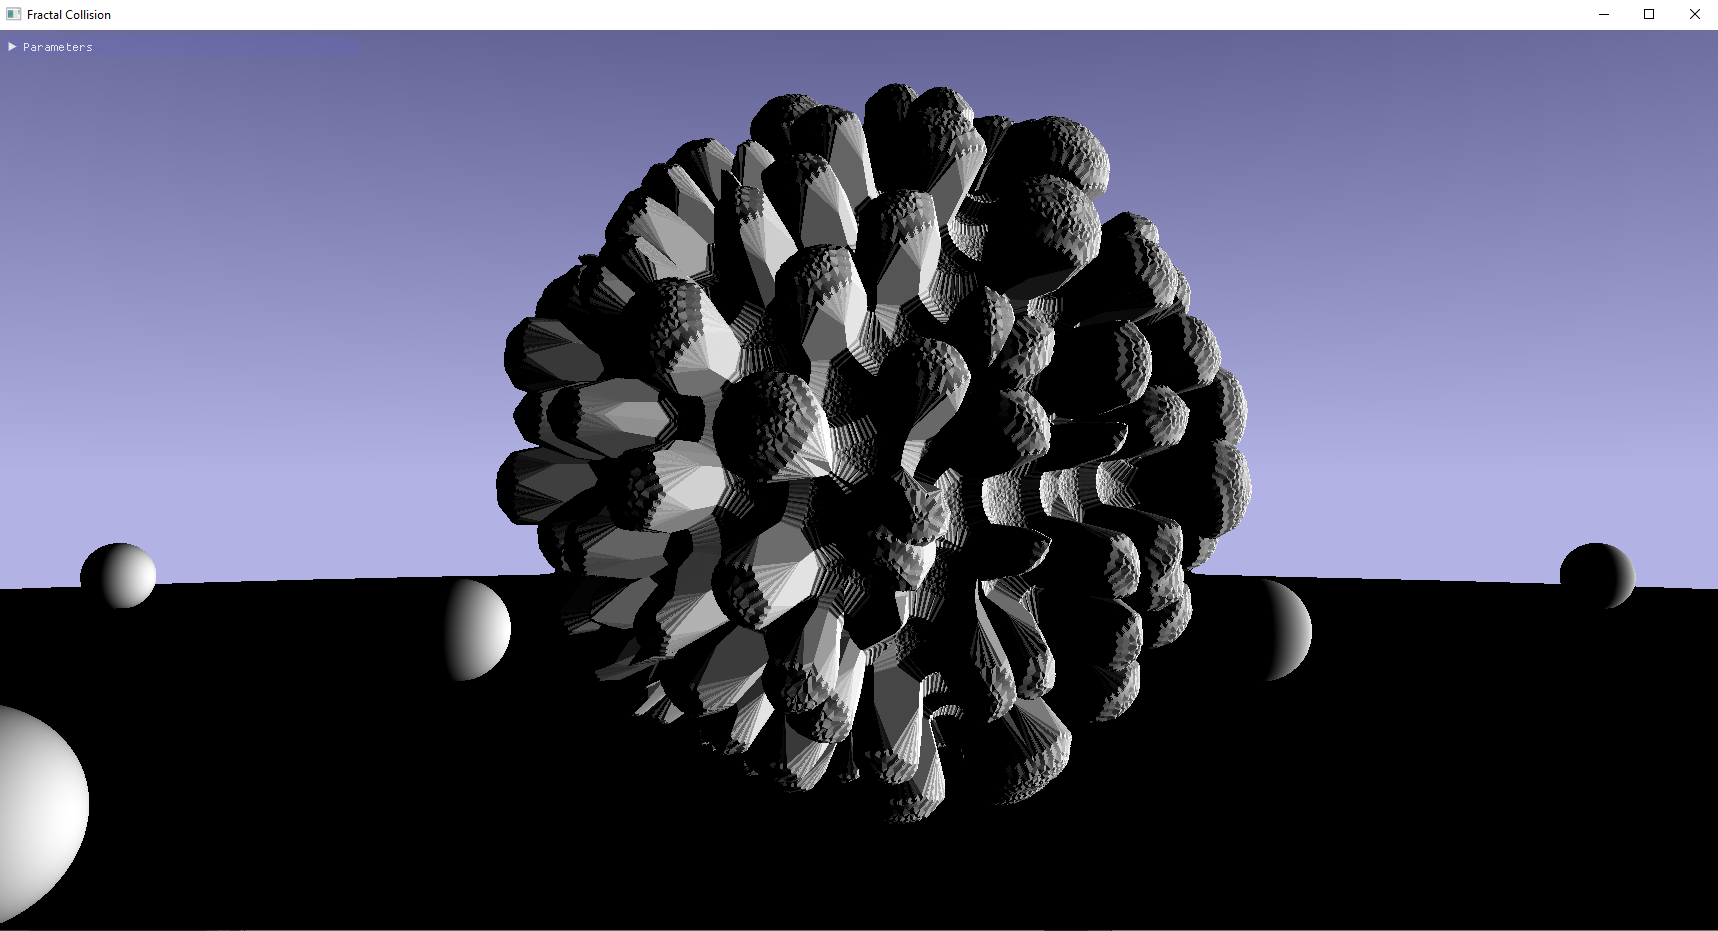
\includegraphics[width=0.3\linewidth]{bac}}
	\vspace{1pt}
	\subfigure[Élfény]{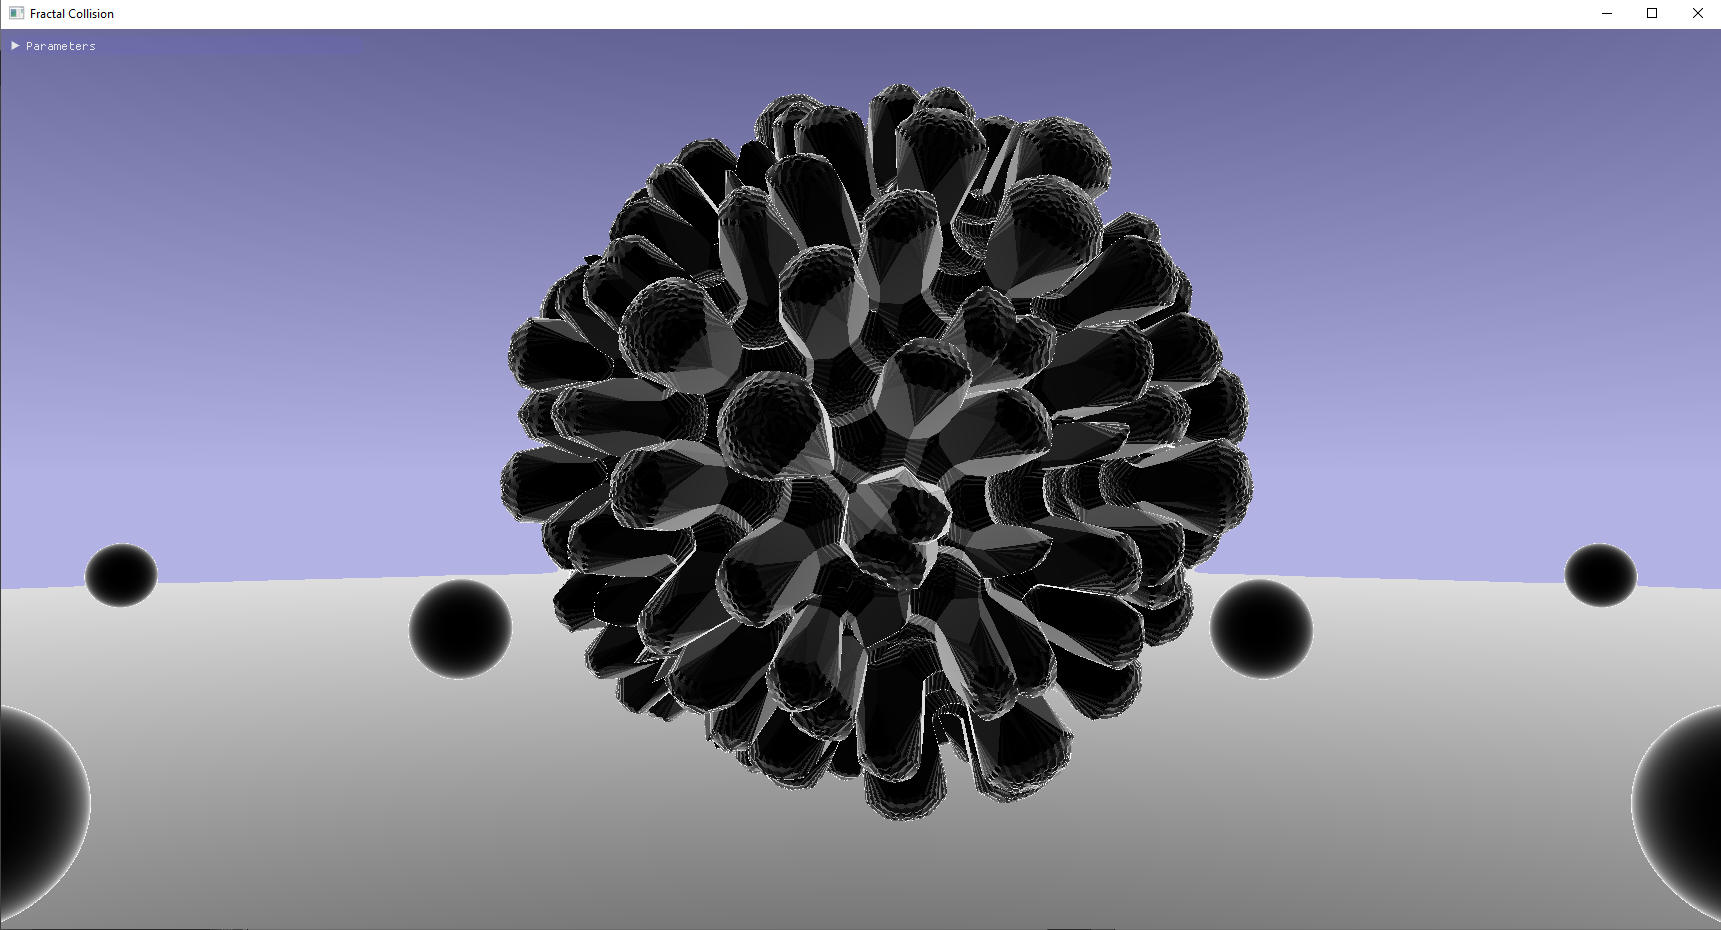
\includegraphics[width=0.3\linewidth]{fre}}
	\hspace{1pt}
	\subfigure[Árnyékalapú tükröződés]{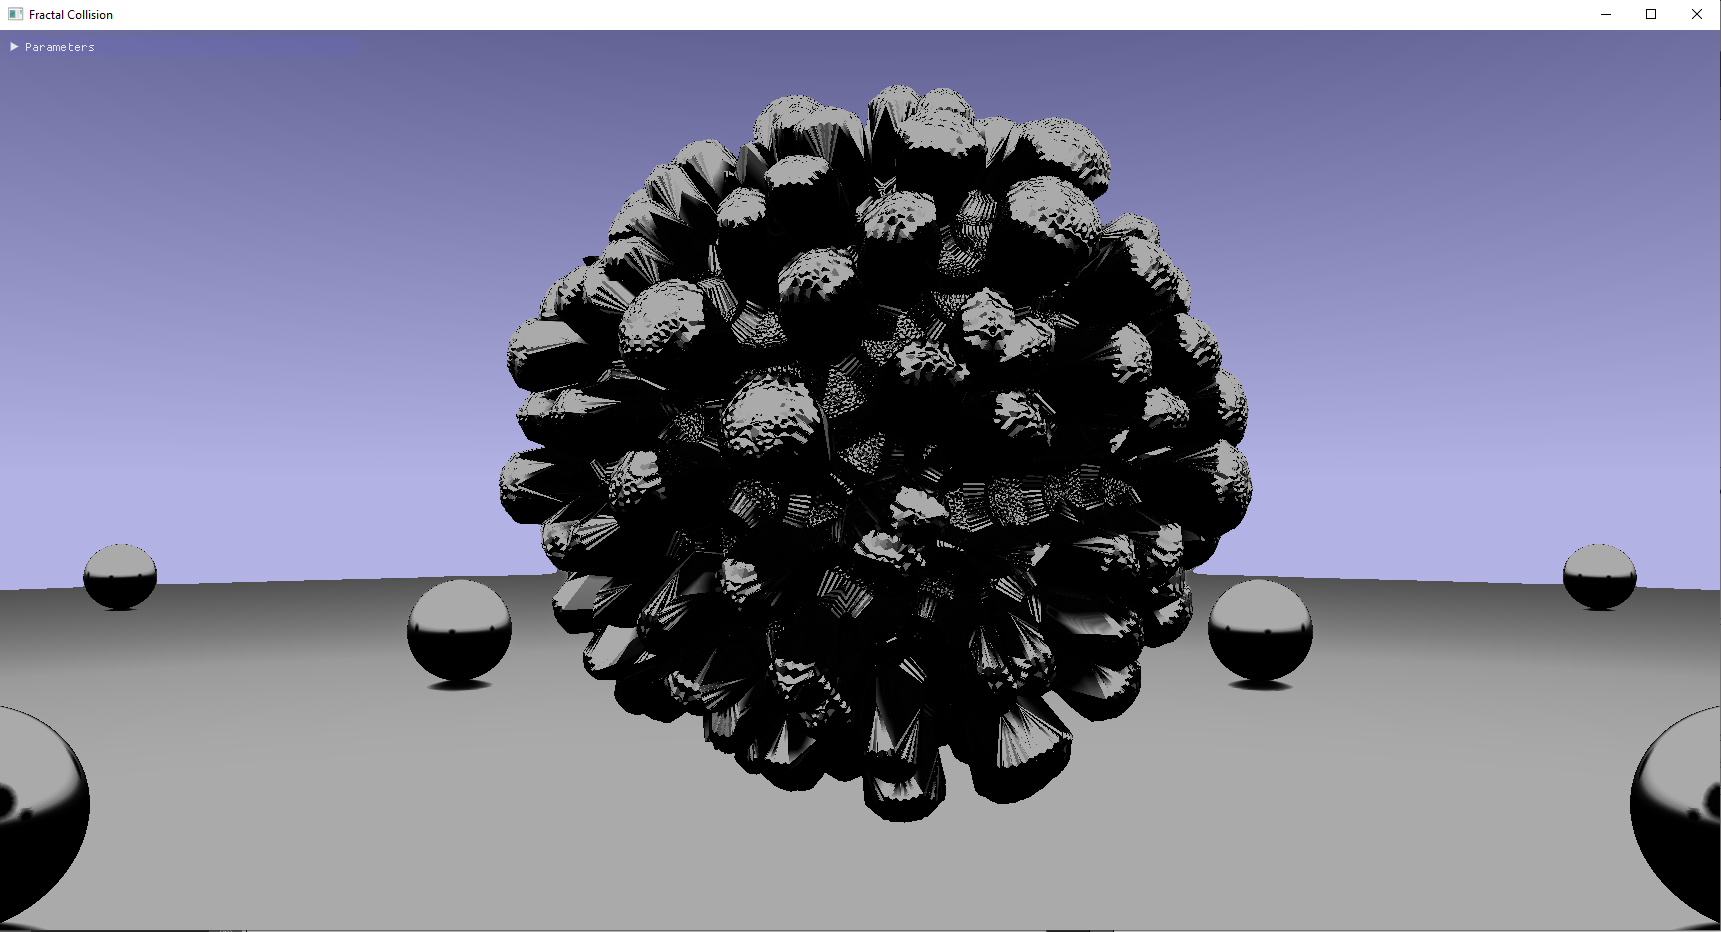
\includegraphics[width=0.3\linewidth]{shadom}}	
	\caption{A fénymodell különböző komponensei}
	\label{fig:lighting}
\end{figure}


\section{Megvalósítás}

A program írása során a Számítógépes Grafika BSc gyakorlat tárgy honlapjának \cite{GrafikaB26:online} projektjei nyújtottak kiindulási alapot. Számos alapvető függvényhívás lett belőlük felhasználva.

\subsection{CMyApp osztály}

Ez a fő osztály. A main.cpp ezen keresztül kezeli le az egér és billentyűzet bemeneteit, szimulálja a fizikát és továbbítja a shaderbe a paramétereket hogy megtörténjen a kirajzolás. A fontosabb függvények külön részletezésre kerülnek.

\subsubsection{bool Init()}

Ebben inicializálódik minden aminek kell. Definiálunk két darab háromszöget melyek egy téglalapot alkotva lefedik majd a teljes ablakot. Ezt a téglalapot fogjuk később a shaderben átszínezni hogy megkapjuk a képet. Az uniform változók memóriacímeit is itt határozzuk meg, valamint a mozgatható labdák pozícióját, méretét és sebességét tartalmazó tömbök is itt kapnak kezdőértékeket.

\subsubsection{void Update()}

Minden képernyőfrissítés előtt lefut, ebben történik a ütközések ellenőrzése és a labdák mozgatása a pozícióik frissítése által. 

A labdák befogott pozíciói -- amikhez akkor közelítenek ha lenyomjuk a szóköz billentyűt -- itt kerülnek meghatározásra a kamerát leíró adatok ismeretében. Meg tudunk határozni egy a kamerából előre, egy jobbra és egy felfelé irányba mutató egységhosszú vektort. Ezek megfelelő kombinációjával és egy időtől és a labdák darabszámától függő forgatási mátrix felhasználásával tudjuk a pozíciójukat egy a kamerához képest fix helyzetű kör mentén beállítani. Mivel az időtől is függ a forgatási mátrix, így ezen kör mentén folyamatosan keringnek.

A labdák hívása és kilövése is itt van megvalósítva. A \textbf{SPACE} nyomva tartásakor labdák az imént kiszámolt pozíciójának és a jelenlegi pozíciójának különbségének konstans-szorosát kapja meg sebességül. Ezáltal minél messzebb van a pozíciótól annál gyorsabban közeledik hozzá. Illetve csak a billentyű nyomva tartásakor frissül egy \textbf{shoot\_time} változóban az idő. 

Ha az aktuális idő és a \textbf{shoot\_time} közötti idő csak kis mértékben tér el akkor tudjuk hogy most lett felengedve a billentyű. Ekkor pedig a kamerából előrefelé mutató vektor konstans-szorosa adódik a labdák sebességéhez.

A labdák \textbf{ütközéseinek megállapításához} a kirajzoláshoz is használt távolságfüggvényt használjuk a vizsgált labda középpontjával. Ha ez a távolság kisebb mint a gömb sugara akkor tudjuk valamivel ütköztünk.

A helyes \textbf{viselkedés megállapításához} ismerünk kell az ütközés pontjában a felületi normálist. A normális kiszámolásához használt módszer (\ref{src:norm}. kódrészlet) a távolságfüggvényt használja így egy egyszerűsítést tehetünk: az ütközési pont helyett a gömb középpontjában számoljuk a felületi normálist! Ezáltal az éleken és sarkokon ahol felületi normális nem igazán értelmezhető, ott is jó viselkedést produkáló vektort fogjuk kapni.

\lstset{caption={A felületi normálist kiszámoló függvény}, label=src:norm}
\begin{lstlisting}[language={C++}]
float RayMarch(vec3 ro, vec3 rd) {
	float dist=0.0;    
    for(int i=0; i<MAX_STEPS; i++) {
    	vec3 p = ro + rd*dist;
        float dS = GetDist(p);
        dist += dS;
        if(dist>MAX_DIST || dS<SURF_DIST ) break;
    }    
    return dist;
}
\end{lstlisting}

Ezután már csak a kapott normálisra kell tükröznünk a vizsgált labdánk sebességvektorát és a megfelelő komponenseit némileg csökkenteni, ezzel szimulálva hogy visszapattanáskor veszít egy keveset az energiájából -- ehhez is a normálist használhatjuk, azért kell komponensenként mert a valóságban ha például elrúgunk ívesen egy focilabdát, akkor annak az vízszintes irányú mozgási energiája jóval kevesebbet csökken visszapattanáskor mint a függőleges irányú. 

Fel kell arra is készülnünk ha a \textbf{labdánk belemegy egy másik objektumba}. Ez többnyire akkor történik meg ha nagyon gyorsan mozog a labda és két ellenőrzés között beleér, vagy ha a labda tartásakor direkt belevisszük egy objektumba. Ha benne vagyunk valamiben akkor frissítjük a pozíció értékét a normális irányába egy kis mértékben.  Ezáltal ha esetleg belekerülne valamibe a labdánk akkor kijön belőle automatikusan.

\begin{figure}[H]
	\centering
	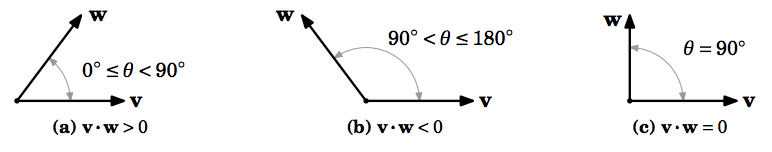
\includegraphics[width=0.8\textwidth]{dot}
	\caption{A skaláris szorzat előjele és a vektorok közötti szög összefüggése}
	\label{fig:dot}
\end{figure}

Mivel tudjuk hogy akár egy másik objektumba is belemehet a labdánk ezért még egy esetre fel kell készülnünk: a másik objektumból kifelé jövet nem szeretnénk hogy ismét tükröződjön a sebességvektor, hiszen akkor állandóan oda-vissza tükröződne és sosem jutna ki a labda. Erre megoldás hogy csak akkor tükrözzük a sebességvektort ha a normálvektorral bezárt szöge \textbf{tompaszög}. Ehhez mindössze a két vektor skaláris szorzatát kell venni és ellenőrizni hogy az eredmény negatív-e.

 
\subsubsection{void Render(int WindowX, int WindowY)} 

Megtörténik a kirajzolás és a shader meghívása. Paraméterként megkapja az ablak méreteit. 


\section{Tesztelés}

A tesztelés során megvizsgáltam hogy a funkciók (\ref{sec:ui}.~fejezet) az elvártaknak megfelelően működne-e. Az ehhez használt számítógép konfiguráció:
\begin{compactitem}
	\item Intel® Core™ i7-8700 CPU
	\item 16 GB RAM
	\item NVIDIA GeForce GTX 1660 GPU
	\item Windows 10 operációs rendszer
\end{compactitem}

\subsection{Működés helyessége}

A következő viselkedéseket ellenőriztem:
\begin{compactenum}
	\item A virtuális kamerát lehet forgatni az \textbf{egérrel};
	\item A virtuális kamera nagyítását lehet állítani a \textbf{CTRL + görgővel} és a csúszkával is;
	\item A virtuális kamerát lehet mozgatni a \textbf{WASD} billentyűkkel;
	\item A mozgás sebességét lehet gyorsítani a \textbf{SHIFT} billentyűvel és állítani a görgővel vagy a csúszkával;
	\item Ha egyszerre gyorsítunk \textbf{SHIFT}-tel és görgővel, a görgő sebessége felülírja a shift gyorsítását;
	\item A fraktál paramétereit át lehet állítani a \textbf{csúszkákkal} és a fraktál ezen értékeknek megfelelően változik;
	\item A \textbf{``Zero values''} gomb hatására megközelíti minden érték a nullát;
	\item A \textbf{``Zero values''} gomb extrém érték esetén: 1000-re állítva egy csúszkát "nullázás" után az értéke 0.423 lett;
	\item A \textbf{``Random values''} gomb valóban véletlenszerű értékeket állít be. Időnként nem látható fraktálokat eredményez;
\end{compactenum}

\subsection{Teljesítmény}

Az alkalmazás erősen GPU igényes.  A futás teljesítményét az alábbi kód segítségével teszteltem:
\lstset{caption={A tesztelést végző kód}, label=src:test}
\begin{lstlisting}[language={C++}]
if (TESTING)
	{
		if (delta_time_counter < avg)
		{
			delta_time_arr[delta_time_counter] = delta_time;
			++delta_time_counter;
		}
		else
		{
			delta_time_counter = 0;
			double avg_delta_time = 0.0;
			for (int i = 0; i < avg; ++i) { avg_delta_time += delta_time_arr[i]; }
			avg_delta_time /= avg;
			printf("Avrage of delta time: %f ms   Iterations: %d   Number of spheres: %d \n", avg_delta_time*1000, iterations, ballCount);
			iterations += 2;
		}
	}
\end{lstlisting}

A kód az \textbf{Update()} függvény alján található. A \textbf{delta\_time} két képfrissítés között eltelt időt jelöli. Ezen kód segítségével \textbf{avg} darab képfrissítési idő átlagát vesszük, ezt kiírjuk az aktuális iterációk száma és mozgatható gömbök száma mellett a terminálablakra, majd ez előbbi értékét megnöveljük kettővel. A tesztek avg=100 értékkel futottak.

A tesztelés idejére ki lett kapcsolva a \textbf{vsync}, hogy ne befolyásolja a mérést. Ha be lenne kapcsolva akkor az 1/60 s = 16.66 ms-nál kisebb kirajzolási idők eredményét nem tudnánk lemérni. Továbbá az a funkció is ideiglenesen ki lett kapcsolva ami alacsony képfrissítési ráta mellett kisebbre veszi az iterációk és gömbök számát.

A kezdeti pozícióhoz képest a kamera nem volt megmozdítva, valamint a tesztben érintett két paraméteren felül más nem lett átállítva a kezdeti alapértelmezettekhez képest. A futás eredményéből készült grafikon \aref{fig:Test1}.~ábrán látható.

\begin{figure}[H]
	\centering
	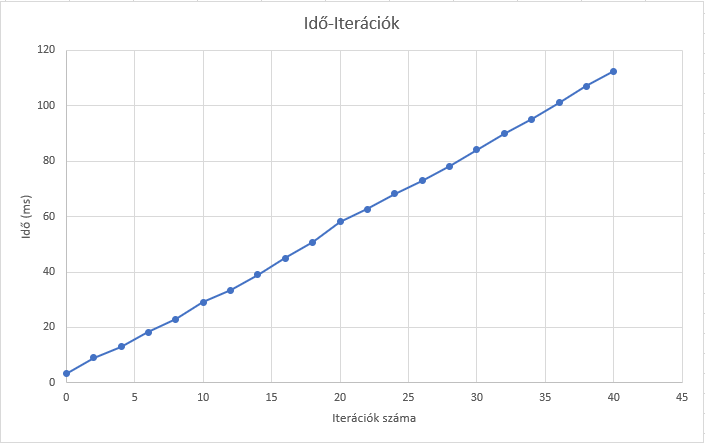
\includegraphics[width=0.8\textwidth,frame]{Test1b}
	\caption{Teljesítményteszt az iterációk számának függvényében}
	\label{fig:Test1}
\end{figure}


Megfigyelhető hogy az iterációk számától lineárisan függ a képfrissítési idő. Bármely két egymást követő sor különbsége 4-6 ms, illetve 10 iterációs eset ideje nagyjából fele a 20-nak és kb. harmada a 30-nak. Az is észrevehető hogy rettentően lelassítja az alkalmazást az iteráció növelése, elég 36-ig felmenni hogy a tesztelői környezeten 10 FPS alá essen a képfrissítési ráta (vagyis 100 ms fölé megy a frissítési idő), ami már határozattan nem folyamatos megjelenítést jelent.

Ha \aref{src:test}.~kód 15. sorát átírjuk \textbf{ballCount += 5} -re akkor azt is meg tudjuk vizsgálni hogy az mozgatható gömbök száma hogyan hat a képfrissítési időre. Ezen futás eredményéből készült grafikont \aref{fig:Test2.}~ábra mutatja.

\begin{figure}[H]
	\centering
	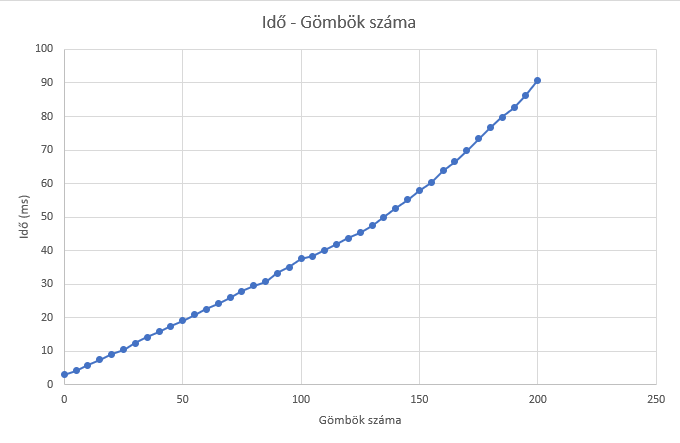
\includegraphics[width=0.8\textwidth,frame]{Test2b}
	\caption{Teljesítményteszt a gömbök számának függvényében}
	\label{fig:Test2}
\end{figure}

Itt is nagyjából lineáris összefüggést tapasztalunk, két egymás utáni érték között 1-3 ms eltérés mutatkozik, illetve az is látható hogy jóval kevesebb hatása van a gömbök számának növelése a teljesítményre. A tesztkonfigurációnak 0 iteráció mellett 40 gömb még nem okoz problémát, ellenben 0 gömb mellett 40 iteráció az előző teszt tanulsága szerint már sokkal inkább.

A gömbök esetében is inkább a megjelenítés okozza a gondot, a \textbf{glDrawArrays()} sor ideiglenes kommentezésével a kirajzolást lényegében megszüntetjük, ám az ütközések modellezését nem befolyásoljuk. Ha ezután újra futtatjuk ez előbbi tesztet, akkor megtudhatjuk hogy a fizika kiszámolása mennyire lassította a kirajzolást. A futás eredményének egy részéből készült grafikon \aref{fig:Test3}.~ábrán látható. 

A grafikonra 350-nél kevesebb gömbhöz tartozó mérési értékek nem szerepelnek, az azokhoz tartozó számolási idő kevesebb mint 1 ms volt. Ez jól mutatja hogy a kirajzolási időhöz képest az ütközések kiszámolása jelentéktelen.

\begin{figure}[H]
	\centering
	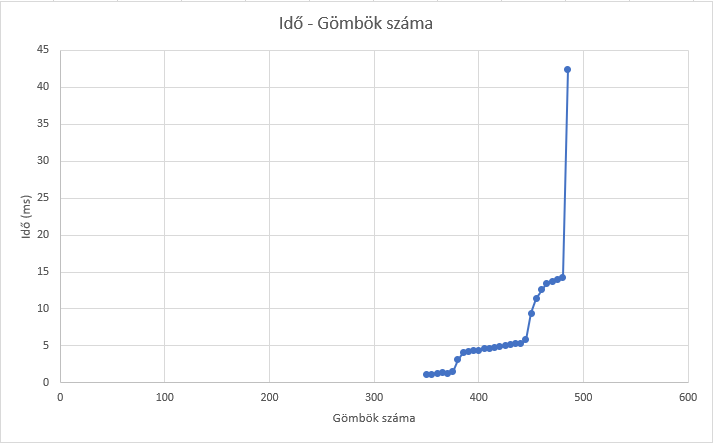
\includegraphics[width=0.8\textwidth,frame]{Test3b}
	\caption{Teljesítményteszt a gömbök számának függvényében, kirajzolás nélkül}
	\label{fig:Test3}
\end{figure}

Az ábra alapján viszont itt már inkább exponenciális összefüggést állapíthatunk meg lineáris helyett. Az utolsó érték 490 gömbbel már 1000 ms volt, de ki lett hagyva az ábrázolás megkönnyítése érdekében. A teszt alatt azonban a magasabb értékek során a processzor összesített kihasználtsága a Windows Task Manager szerint 14\%-os volt, és egyik szál sem mutatott állandó teljes terhelést.  A jelenség pontos forrása ismeretlen, de mivel csak extrém körülmények között jelentkezik, így nem lett sok idő fordítva az ok felkutatására.